\subsection{User interfaces}
The interface of MyTaxiService can be for web application and mobile application. Here will be presented some of the most important pages and screens of MyTaxiService.

\paragraph{Log in:}
	In the figure below is shown the MyTaxiService's homepage
	\begin{center}
		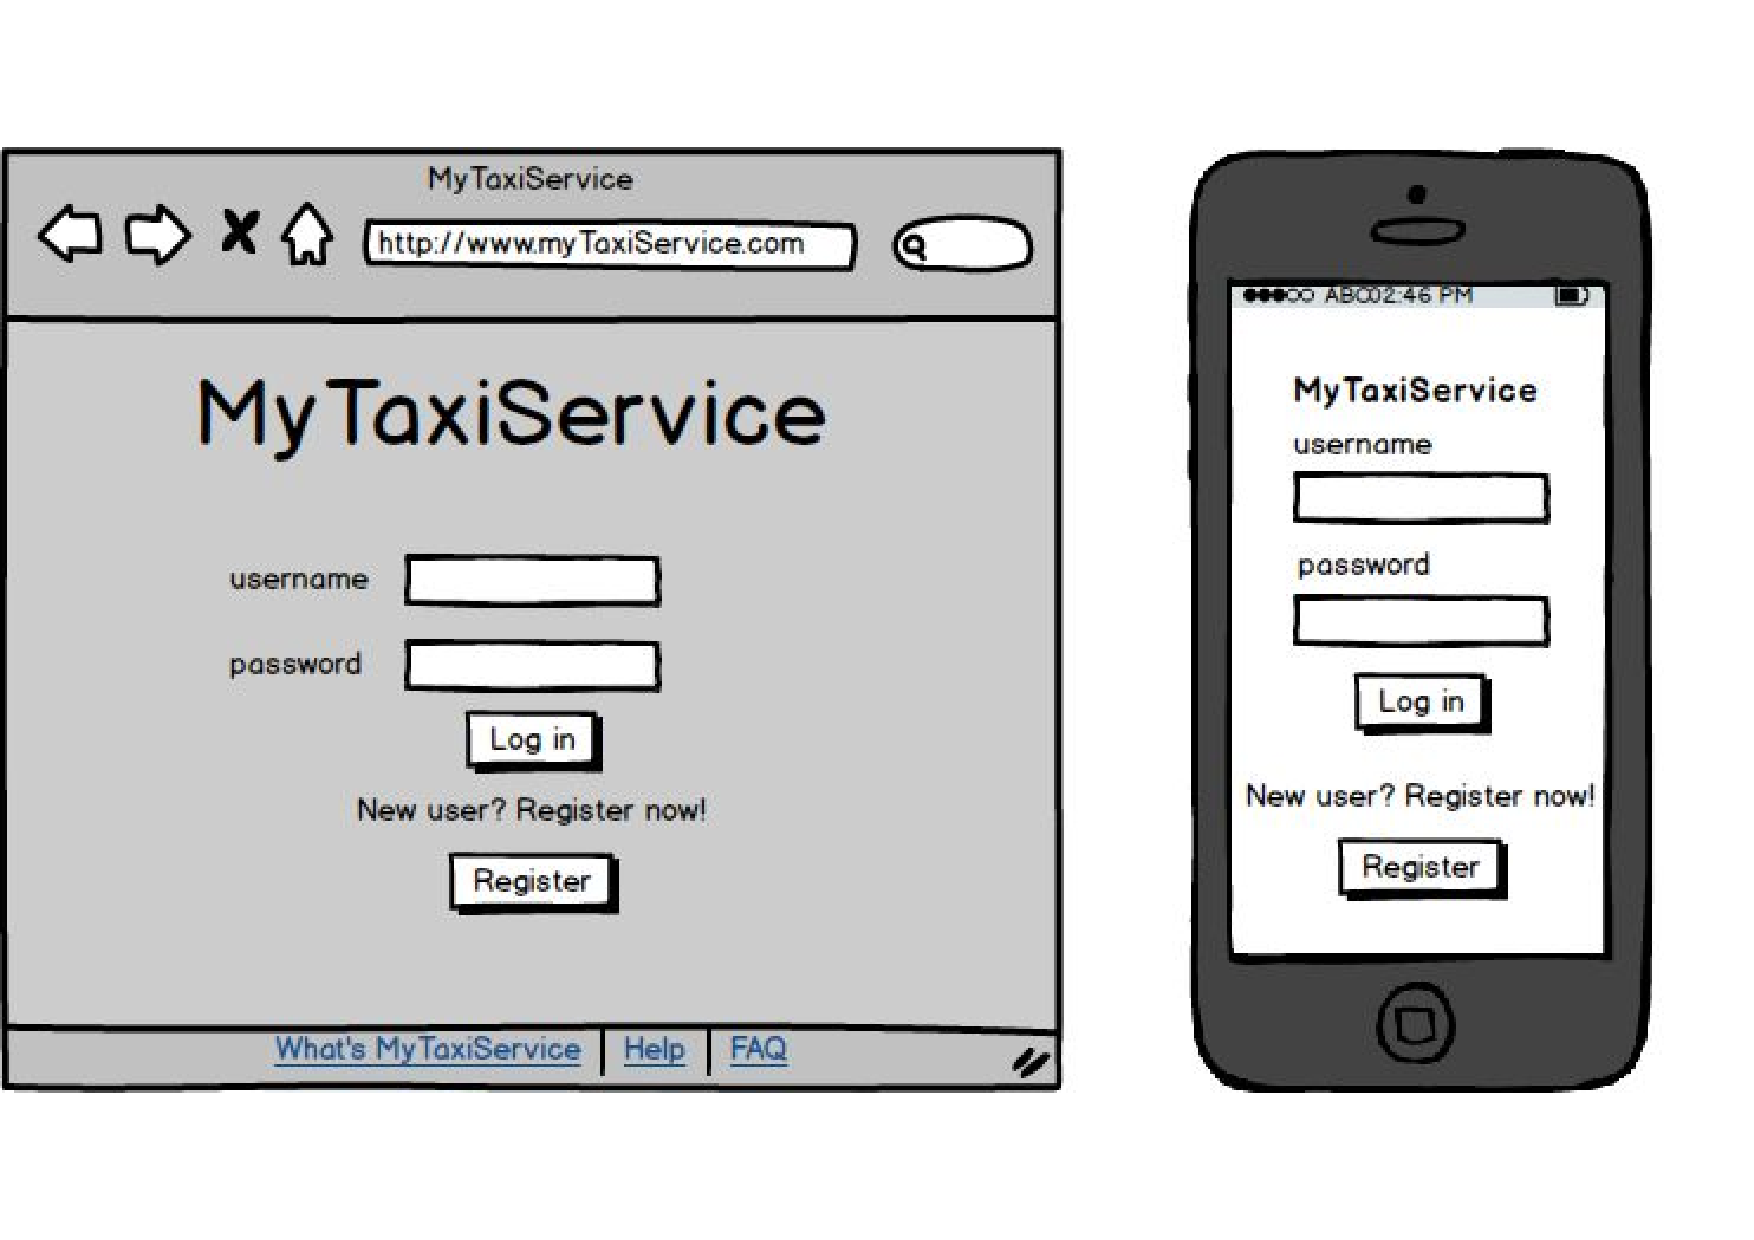
\includegraphics[width=\textwidth]{mockup/login.pdf}
	\end{center}
	
\paragraph{Registration:}
	Here the visitor can sig up to the application
\begin{center}
	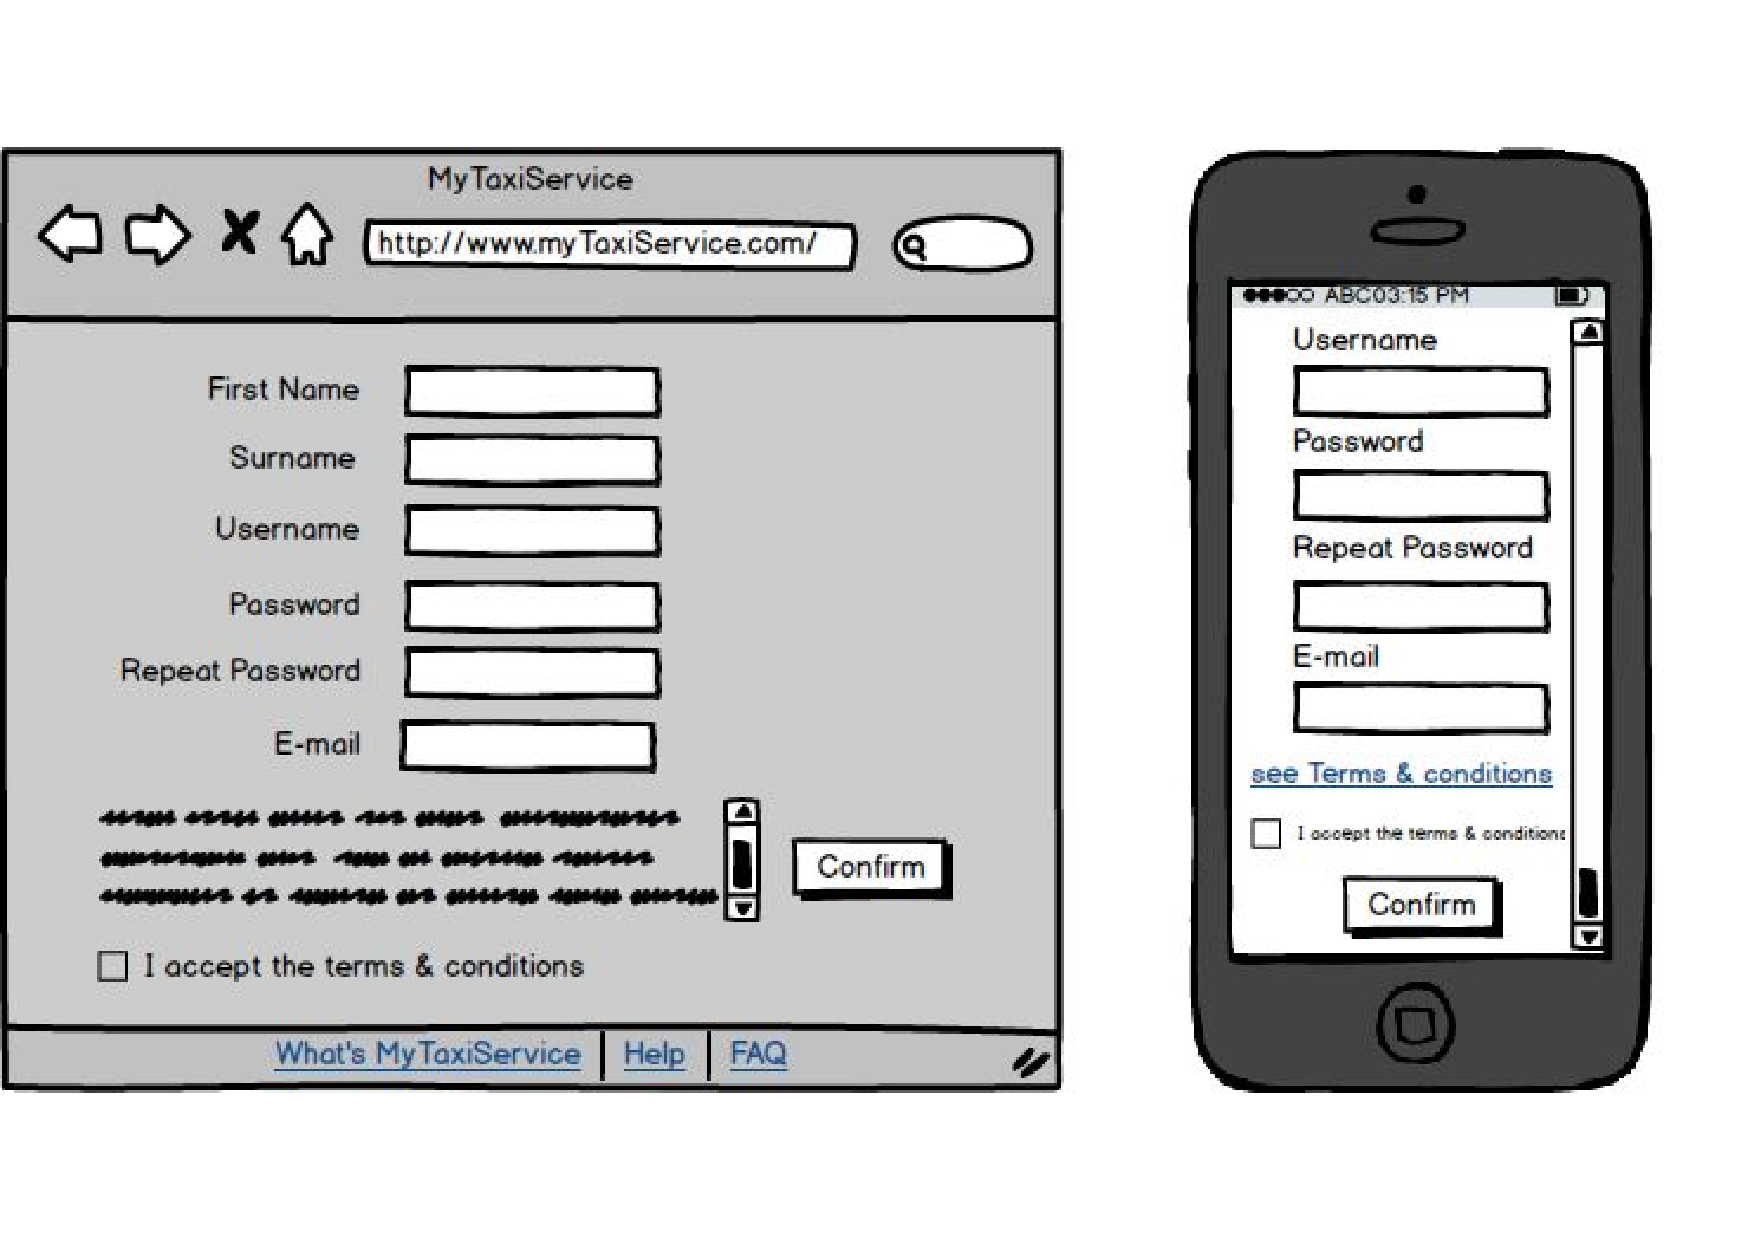
\includegraphics[width=\textwidth]{mockup/registration.pdf}
\end{center}

\paragraph{Passenger view:}
This is the view of the passenger
\begin{center}
	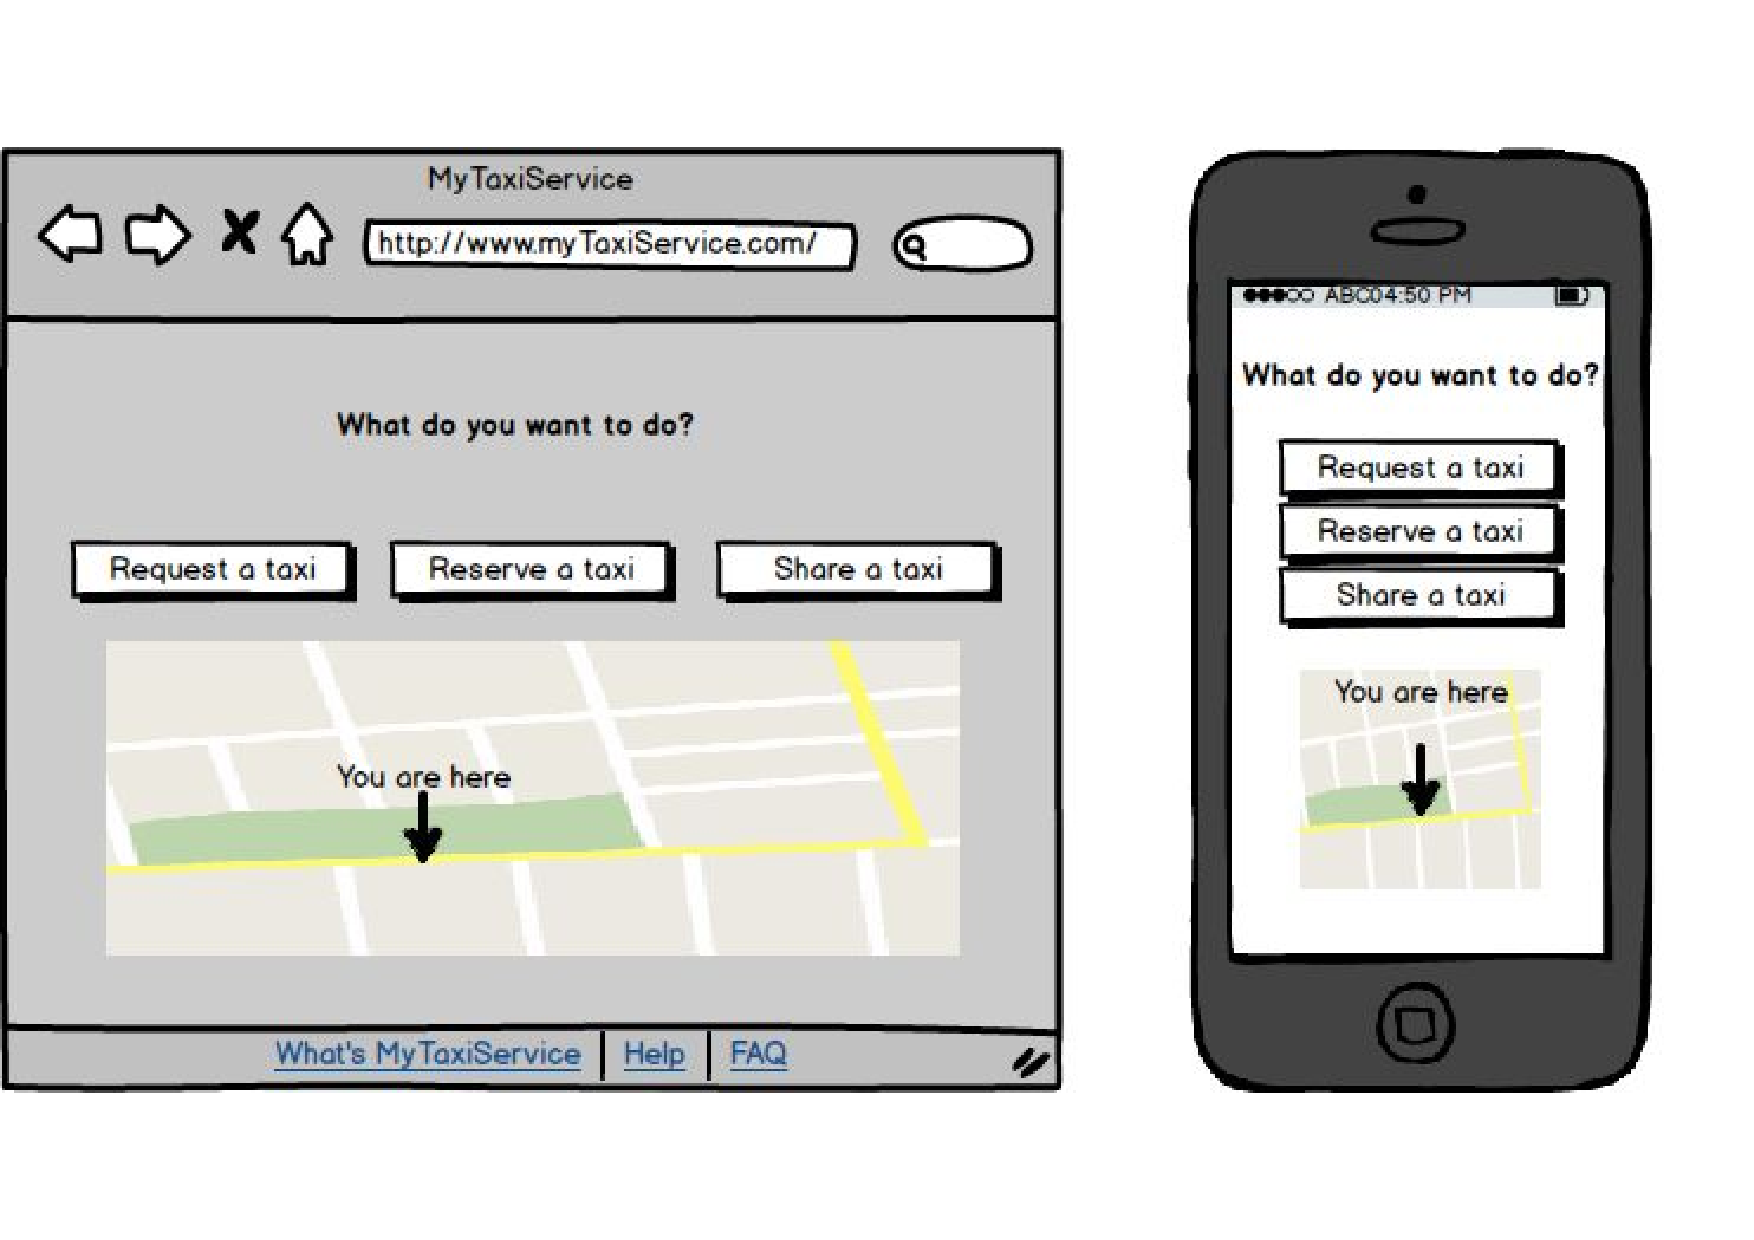
\includegraphics[width=\textwidth]{mockup/passengerFunctions.pdf}
\end{center}

\paragraph{Taxi driver view:}
This is the view of the taxi driver
\begin{center}
	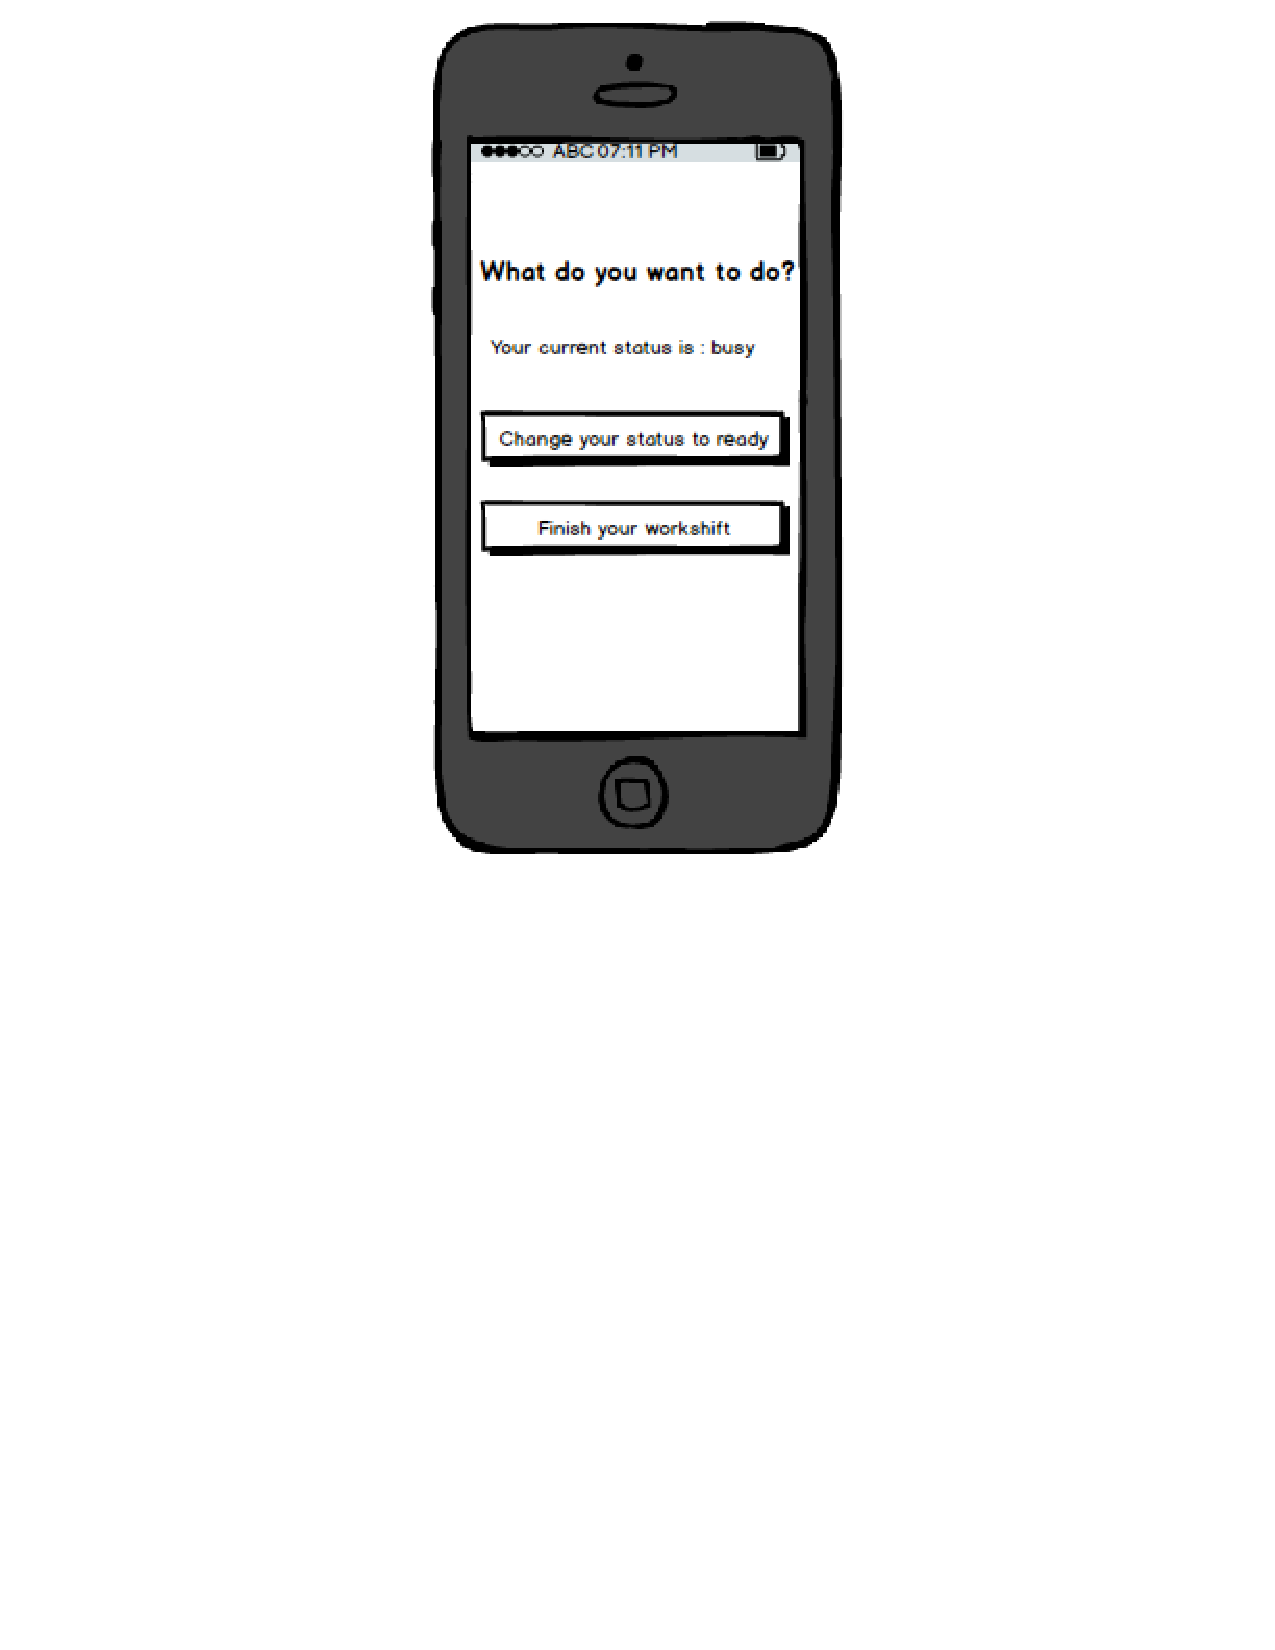
\includegraphics[width=\textwidth]{mockup/taxiDriverFunctions.pdf}
\end{center}

\paragraph{Taxi driver notification:}
This is the notification that the taxi driver, choosen by the system, see when a passenger request a ride.
\begin{center}
	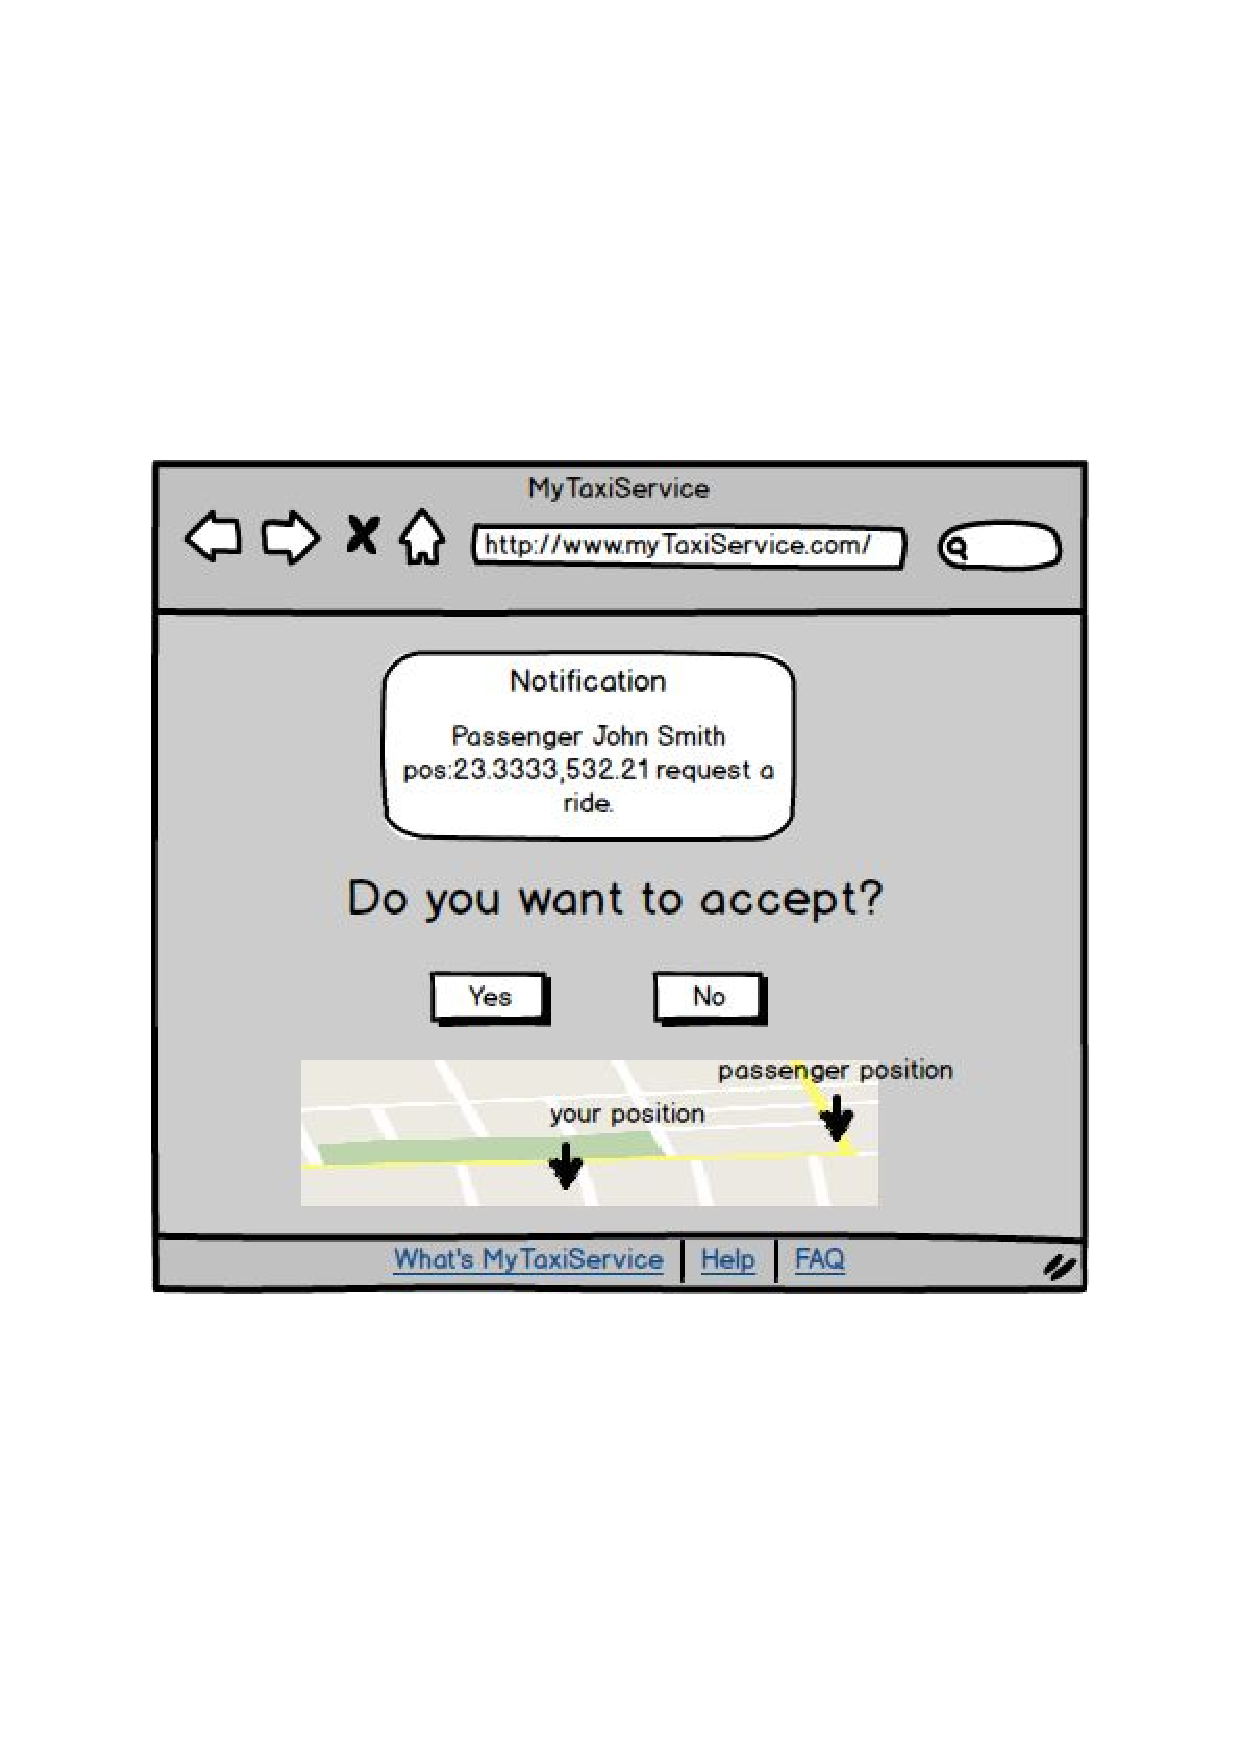
\includegraphics[width=\textwidth]{mockup/taxiDriverNotification.pdf}
\end{center}
\paragraph{Passenger notification :}
This is the notification that the passenger see when a taxi accept the ride
\begin{center}
	\includegraphics[width=\textwidth]{mockup/PassengerNotification.pdf}
\end{center}

\subsection{API interfaces}
\subsection{Hardware interfaces}
MyTaxiService doesn't support any hardware interfaces. 
\subsection{Software interfaces}
\subsection{Communication interfaces}

